\documentclass{standalone}
\usepackage{tikz}
\usepackage{ctex,siunitx}
\setCJKmainfont{Noto Serif CJK SC}
\usepackage{tkz-euclide}
\usepackage{amsmath}
\usetikzlibrary{patterns, calc,3d}
\usetikzlibrary {decorations.pathmorphing,decorations.pathreplacing,decorations.shapes}
\begin{document}
\small
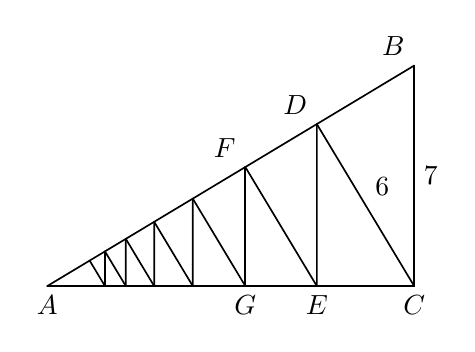
\begin{tikzpicture}[>=latex,scale=0.8]
  \tkzDefPoints{0/0/C,0/3.5/B,3/0/X}
  \tkzDefLine[tangent from=B](C,X)\tkzGetPoints{D'}{D}
  \tkzInterLL(C,X)(B,D)\tkzGetPoint{A}
  \tkzDefPointsBy[projection=onto A--C](D){E}
  \tkzDefPointsBy[projection=onto A--B](E){F}
  \tkzDefPointsBy[projection=onto A--C](F){G}
  \tkzDefPointsBy[projection=onto A--B](G){H}
  \tkzDefPointsBy[projection=onto A--C](H){I}
  \tkzDefPointsBy[projection=onto A--B](I){J}
  \tkzDefPointsBy[projection=onto A--C](J){K}
  \tkzDefPointsBy[projection=onto A--B](K){L}
  \tkzDefPointsBy[projection=onto A--C](L){M}
  \tkzDefPointsBy[projection=onto A--B](M){N}
  \tkzDefPointsBy[projection=onto A--C](N){O}
  \tkzDefPointsBy[projection=onto A--B](O){P}
  \tkzDrawSegments[semithick](C,A B,A B,C C,D D,E E,F F,G G,H H,I I,J J,K K,L L,M M,N N,O O,P)
  \tkzLabelPoints(A,C,E,G)
  \tkzLabelPoints[above left](B,D,F)
  \tkzLabelLine[pos=0.5,above right](C,D){6};
  \tkzLabelLine[pos=0.5,right](C,B){7};
\end{tikzpicture}
\end{document}